\documentclass[12pt]{article}

\usepackage[russian]{babel}
\usepackage{geometry}

\usepackage{graphicx} % вставка изображений
\usepackage{caption} % описание изображений

%различные цветовые модели
\usepackage[usenames]{color}
\usepackage[dvipsnames,table]{xcolor}
\usepackage{colortbl}

\usepackage{tikz}
\usetikzlibrary{shapes, arrows}
\usepackage{varwidth}
\usepackage{ifthen}

\usepackage{enumitem}

\usepackage{multicol} % вставка изображений в две колонки
\usepackage{makecell} % вставка изображений в две колонки


%циклы foreach в tikz и создание переменных внутри этого окружения
\usepackage{pgffor}
\usepackage{pgfmath}

\usepackage{xifthen}

\usepackage{afterpage}

\usepackage{amssymb}
\usepackage{amsmath}

\usepackage{hyperref}

%\usepackage[utf8]{inputenc}

\tikzstyle{connector} = [draw, -latex']
\tikzstyle{line} = [draw, -]
\tikzstyle{dashed} = [draw, -, dash pattern=on 5pt off 5pt]


\usepackage{listings}
\usepackage{listingsutf8}
\usepackage[T2A]{fontenc}
\newcommand{\listingsttfamily}{\usefont{T2A}{PTMono-TLF}{m}{n}}

\lstset{
	language=C,                % choose the language of the code
	numbers=left,                   % where to put the line-numbers
	stepnumber=1,                   % the step between two line-numbers.        
	numbersep=5pt,                  % how far the line-numbers are from the code
	backgroundcolor=\color{black},  % choose the background color. You must add \usepackage{color}
	commentstyle=\color{Gray},
	basicstyle=\listingsttfamily\color{Gray},
	keywordstyle=\color{BurntOrange},
	stringstyle=\color{YellowGreen},
	showspaces=false,               % show spaces adding particular underscores
	showstringspaces=false,         % underline spaces within strings
	showtabs=false,                 % show tabs within strings adding particular underscores
	tabsize=4,                      % sets default tabsize to 2 spaces
	captionpos=b,                   % sets the caption-position to bottom
	breaklines=true,                % sets automatic line breaking
	breakatwhitespace=true,         % sets if automatic breaks should only happen at whitespace
	title=\lstname, 
	inputencoding=utf8,                % show the filename of files included with \lstinputlisting;
	extendedchars=\true,
	keepspaces=true
}

\geometry{top=2cm, bottom=2cm, left=3cm, right=1.5cm}
\textheight=24cm
\textwidth=18cm
\flushbottom 

\oddsidemargin=0pt 
\topmargin=-1.5cm 
\parskip=0.25cm
\parindent=24pt 

\tolerance=2000 

\setcounter{secnumdepth}{0}

\setlist[1]{noitemsep} % sets the itemsep and parsep for all level two lists to 0

\begin{document}
	\begin{center}
		{\parskip=1cm
			МИНИСТЕРСТВО НАУКИ И ВЫСШЕГО ОБРАЗОВАНИЯ РОССИЙСКОЙ ФЕДЕРАЦИИ
			
			ФЕДЕРАЛЬНОЕ ГОСУДАРСТВЕННОЕ БЮДЖЕТНОЕ ОБРАЗОВАТЕЛЬНОЕ УЧРЕЖДЕНИЕ ВЫСШЕГО ОБРАЗОВАНИЯ
			
			{\bf«БЕЛГОРОДСКИЙ ГОСУДАРСТВЕННЫЙ ТЕХНОЛОГИЧЕСКИЙ УНИВЕРСИТЕТ им. В. Г. Шухова»\\(БГТУ им. В. Г. Шухова)}
			
			\begin{figure}[bh]
				\noindent\centering{
					
\includegraphics[width=100mm]{images/start_logo.png}
					\captionsetup{labelformat=empty}
				}
			\end{figure}
			Кафедра программного обеспечения вычислительной техники и автоматизированных систем
		}
		
		{\Large 
			\vspace{1cm}
			{\parskip=0.25cm 
				{\bf Лабораторная работа №4.3}
				
				по дисциплине: «Дискретная математика»
				
				по теме: {\bf Связность}
			}
		}
	\end{center}	
	\begin{flushleft}
		{\leftskip=10cm
			{\vspace{3cm} Выполнил/a: ст. группы ПВ-231}
			
			Чупахина София Александровна
			
			Проверил: Рязанов Юрий Дмитриевич
			
		}
	\end{flushleft}
	\begin{center}
		{\parskip=3cm Белгород, 2024}
	\end{center}
	\newpage

	\tableofcontents
	
	\newpage
	
	\section{Задание 1}
	\label{task1}
	{\bf Текст задания:} Реализовать алгоритм Краскала построения покрывающего леса. 
	
	Реализуем алгоритм в том виде, в котором это предложено сделать в лекции. В начале работы алгоритма создадим массив bunches, число элементов в котором равно числу элементов в графе вообще. Этот массив отображает, в каком букете какая вершина графа находится на данный момент формирования леса: если i-тый, начиная отсчет с нуля, элемент в массиве равен n, значит, вершина со значением i+1 находится в букете с номером n. Следует отметить, что в процессе формирования дерева номера букетов не обязательно идут от единицы до их конечного количества; их номера призваны только давать понять, в одном или разных букетах находятся вершины. Циклом пробегая все элементы массива, будем задавать им номера от 1 до максимального значения среди вершин графа. После этого с помощью двух вложенных циклов будем пробегать по элементам матрицы смежности данного графа, перебирая пары значений вершин. Для каждого элемента буем проверять, равен ли он единице (то есть смежна ли рассматриваемая пара вершин) и различны ли значения массива bunches на позициях, соответствующих этим элементам (то есть различны ли номера букетов, которым принадлежат рассматриваемые вершины). Если оба этих условия выполняются, то ребро между рассматриваемыми вершинами вносится в формируемый граф: в матрице смежности устанавливаются в 1 элементы, соответствующие данной паре вершин (без учета порядка). Затем происходит слияние букетов: запоминается номер букета для одной из вершин, а затем с помощью цикла все элементы массива bunches с этим значением заменяются на номер букета второй вершины.
	
	\lstinputlisting{graphs/Kraskal.c} 
	
	\section{Задание 2}
	\label{task2}
	
	{\bf Текст задания:} Используя алгоритм Краскала, разработать и реализовать алгоритм решения задачи (см. варианты заданий).
	
	{\bf Задача для варианта 6: } Найти все множества вершин, исключение которых из связного графа разбивает его на две связные компоненты, причем каждая компонента не содержит изолированных вершин.
	
	Поступим следующим образом. Будем находить все возможные множества вершин для данного графа, для каждого из этих множеств строить граф, из которого эти вершины (условно) исключены, и для построенного графа определять, является ли он состоящим из двух связных компонент и нет ли в нем изолированных вершин. Первым делом, добавим в файл функции для работы с массивами --- последовательностями целых чисел (в прошлых лабораторных работах мы представляли и упорядоченные последовательности, и множества вершин именно так). Если быть точнее, это функция вывода множества вершин на экран и функция, определяющая, входит ли в множество некоторый элемент.
	
	\lstinputlisting[linerange={1-22}]{graphs/task_6_final.c} 
	
	Как мы будем перебирать все возможные множества вершин? Очевидно, это будут подмножества от множества всех вершин данного графа. Подмножество можно задать двоичным вектором, где количество разрядов равно количеству элементов исходного множества, и каждый разряд обозначает, входит ли в подмножество элемент исходного множества, соответствующий данному разряду (элементам присваиваются порядковые номера, и разряды двоичных векторов соотносятся с элементами по их номерам). если множество имеет мощность $|M|$, то и двоичные вектора будут иметь длину $|M|$, а количество возможных значений этих векторов будет равно $2^{|M|}$. Значит, чтобы перебрать все возможные подмножества вершин, нам нужно перебрать все числа от 0 (все нули, ни один элемент не входит в подмножество) до $2^{|M|}-1$ (все единицы, все элементы входят в подмножество). Впрочем, эти крайние значения можно и опустить, потому что понятно: не исключив ни одной вершины, мы не сможем разбить массив на две компоненты, а при исключении всех вершин полученный граф вообще компонент иметь не будет. 
	
	Для такой стратегии необходимо написать функцию, переводящуюю двоичный вектор (то есть обычное целое число) в последовательность целых чисел (значения отдельных разрядов в целом числе получаем с помощью побитовых операций):
	
	\lstinputlisting[linerange={24-35}]{graphs/task_6_final.c} 
	
	Как уже было сказано, после получения каждого подмножества мы будем строить для него подграф исходного графа, в котором данные вершины удалены. В теле функции, выполняющей эту операцию, результирующий граф создается с тем же набором вершин (матрица смежности не меняет размерность), но без ребер. Все ребра исходного графа перебираются парой вложенных циклов; соответствующие им значения в матрице смежности переносятся в результирующий граф, только если ни одна из вершин не входит в последовательность, вершины из которой должны быть исключены.
	
	\lstinputlisting[linerange={37-48}]{graphs/task_6_final.c} 
	
	Для построенного графа необходимо определить два свойства. Первое --- разбит ли он ровно на две связные компоненты? В этом нам и поможет алгоритм Краскала для построения покрывающего леса. Для одного исходного графа может быть построено несколько покрывающих деревьев/лесов, но количество ребер в них постоянно, не зависит от порядка, в котором перебирались ребра исходного графа при построении, и равно разности количества вершин и связных компонент исходного графа. Так что построив покрывающий лес по этому алгоритму, нужно лишь посчитать ребра в получившемся графе и сделать вывод, равно ли оно количеству вершин исходного графа минус два (ведь по условию задачи, граф должен быть разбит на две связных компоненты).
	
	Алгоритм Краскала уже был реализован в задании 1. Остается только реализовать функцию подсчета ребер в графе.
	
	\lstinputlisting[linerange={50-58}]{graphs/task_6_final.c} 
	
	Второе поставленное в задаче условие --- отсутствие изолированных вершин. Здесь можно воспользоваться тем фактом, что строки в матрице смежности в данной реализации графов кодируются целыми числами (и разбиваются на нули и единицы побитовыми операциями). Если вершина изолирована, значит, она не имеет инцидентных ей ребер, соответствующая ей строка в матрице не содержит ни одной единицы и кодируется нулем. Для подсчета количества изолированных вершин в графе нужно лишь перебрать в цикле все строки матрицы и вернуть количество нулевых.
	
	Важно отметить: нам необходимо именно считать количество изолированных вершин, а не просто выносить вердикт о их наличии/отсутствии. Ведь после удаления вершин из графа (а фактически --- удаления всех ребер, которым они были инциденты) информация о их существовании по-прежнему будет храниться в матрице смежности, и они будут считываться этим алгоритмом как изолированные. Значит, чтобы полученный граф удовлетворяло условию, необходимо, чтобы количество изолированных вершин в нем было равно количеству удаленных, но не превышало его.
	
	\lstinputlisting[linerange=60-68]{graphs/task_6_final.c} 
	
	Совместим все вышеописанные шаги и условия в результирующую функцию, перебирающую подмножества от исходного множества вершин графа, строящую подграф, из которого эти вершины удалены, и выводит на экран подмножество вершин, если полученный граф удовлетворяет условиям. 
	
	В целях уменьшения количества перебираемых подмножеств можно установить еще одно условие: начинать проверку условий для этого подмножества, только если количество вершин после удаления больше или равно четырем. Ведь меньшее количество вершин нельзя разбить на две связных компоненты так, чтобы хотя бы одна из них не оказалась изолированной.
	
	\lstinputlisting[linerange=70-84]{graphs/task_6_final.c} 

	
	\section{Задание 3}
	\label{task3}

	{\bf Текст задания:} Подобрать тестовые данные. Результат представить в виде диаграммы графа. 
	
	Вручную составим несколько графов, постаравшись отобразить в них как некоторые общие случаи, так и продемонстрировав показательно простые примеры. Затем будем создавать аналогичные графы в программе и запускать для них написанную функцию.
	
	Для задания графа с помощью литералов определим в файле тестирования уже использовавшуюся ранее в лаораторных работах по графам функцию graph\_createFromMatrix:
	
	\lstinputlisting[linerange=1-15]{graphs/tests.c} 
	
	Начнем с графа, вырождающегося в линейную последовательность.
	
	\begin{tikzpicture}{line width=3pt}
		\def\step{1.25}
		\node[circle, draw=black] at (-3*\step, -\step) (knot1) {1};
		\node[circle, draw=black] at (-2*\step, -0.66*\step) (knot2) {2};
		\node[circle, draw=black] at (-1*\step, -0.33*\step) (knot3) {3};
		\node[circle, draw=black] at (1*\step, -0.33*\step) (knot4) {4};
		\node[circle, draw=black] at (2*\step, -0.66*\step) (knot5) {5};
		\node[circle, draw=black] at (3*\step, -\step) (knot6) {6};
		
		\path[line, line width = 1.25pt] (knot1) -- (knot2);
		\path[line, line width = 1.25pt] (knot2) -- (knot3);
		\path[line, line width = 1.25pt] (knot3) -- (knot4);
		\path[line, line width = 1.25pt] (knot4) -- (knot5);
		\path[line, line width = 1.25pt] (knot5) -- (knot6);
	\end{tikzpicture}
	
	Удаление его крайних вершин (имеющих степень связности 1) не приведет к разбиению на 2 компоненты; удаление вершин, смежных крайним, приведет к формированию компонент из изолированных вершин. Но вершины между теми, что смежны с крайними, удалять можно, как по одной, так и по несколько за раз, если они идут подряд; плюс, если удаление какой-то вершины приводит к формированию компоненты, где больше двух вершин, можно удалить в них крайние.
	
	\begin{tabular}{|c|c|}
	\hline
	Удаленные вершины & Полученный граф \\
	\hline
	3 & \begin{tikzpicture}{line width=3pt}
		\def\step{1.25}
		\node[circle, draw=black] at (-3*\step, -\step) (knot1) {1};
		\node[circle, draw=black] at (-2*\step, -0.66*\step) (knot2) {2};
		\node[circle, draw=black] at (1*\step, -0.33*\step) (knot4) {4};
		\node[circle, draw=black] at (2*\step, -0.66*\step) (knot5) {5};
		\node[circle, draw=black] at (3*\step, -\step) (knot6) {6};
		
		\path[line, line width = 1.25pt] (knot1) -- (knot2);
		\path[line, line width = 1.25pt] (knot4) -- (knot5);
		\path[line, line width = 1.25pt] (knot5) -- (knot6);
	\end{tikzpicture} \\
	\hline
	4 & \begin{tikzpicture}{line width=3pt}
		\def\step{1.25}
		\node[circle, draw=black] at (-3*\step, -\step) (knot1) {1};
		\node[circle, draw=black] at (-2*\step, -0.66*\step) (knot2) {2};
		\node[circle, draw=black] at (-1*\step, -0.33*\step) (knot3) {3};
		\node[circle, draw=black] at (2*\step, -0.66*\step) (knot5) {5};
		\node[circle, draw=black] at (3*\step, -\step) (knot6) {6};
		
		\path[line, line width = 1.25pt] (knot1) -- (knot2);
		\path[line, line width = 1.25pt] (knot2) -- (knot3);
		\path[line, line width = 1.25pt] (knot5) -- (knot6);
	\end{tikzpicture} \\
	\hline
	
	1, 4 & \begin{tikzpicture}{line width=3pt}
		\def\step{1.25}
		\node[circle, draw=black] at (-2*\step, -0.66*\step) (knot2) {2};
		\node[circle, draw=black] at (-1*\step, -0.33*\step) (knot3) {3};
		\node[circle, draw=black] at (2*\step, -0.66*\step) (knot5) {5};
		\node[circle, draw=black] at (3*\step, -\step) (knot6) {6};
		
		\path[line, line width = 1.25pt] (knot2) -- (knot3);
		\path[line, line width = 1.25pt] (knot5) -- (knot6);
	\end{tikzpicture} \\
	\hline
	3, 4 & \begin{tikzpicture}{line width=3pt}
		\def\step{1.25}
		\node[circle, draw=black] at (-3*\step, -\step) (knot1) {1};
		\node[circle, draw=black] at (-2*\step, -0.66*\step) (knot2) {2};
		\node[circle, draw=black] at (2*\step, -0.66*\step) (knot5) {5};
		\node[circle, draw=black] at (3*\step, -\step) (knot6) {6};
		
		\path[line, line width = 1.25pt] (knot1) -- (knot2);
		\path[line, line width = 1.25pt] (knot5) -- (knot6);
	\end{tikzpicture} \\
	\hline
	
	3, 6 & \begin{tikzpicture}{line width=3pt}
		\def\step{1.25}
		\node[circle, draw=black] at (-3*\step, -\step) (knot1) {1};
		\node[circle, draw=black] at (-2*\step, -0.66*\step) (knot2) {2};
		\node[circle, draw=black] at (1*\step, -0.33*\step) (knot4) {4};
		\node[circle, draw=black] at (2*\step, -0.66*\step) (knot5) {5};

		\path[line, line width = 1.25pt] (knot1) -- (knot2);
		\path[line, line width = 1.25pt] (knot4) -- (knot5);

	\end{tikzpicture} \\
	\hline
	\end{tabular}
	
	Функция выведет те же наборы вершин, что и в первом столбце таблицы:
	
	\lstinputlisting[linerange={17-29, 84}]{graphs/tests.c} 
	
	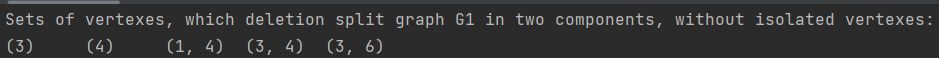
\includegraphics[width=170mm]{images/G1.png} 
	
	Следом рассмотрим граф, являющийся деревом.
	
	\begin{tikzpicture}{line width=3pt}
		\def\step{1.25}
		\node[circle, draw=black] at (-2*\step, 0) (knot1) {1};
		\node[circle, draw=black] at (-1*\step, 0) (knot2) {2};
		\node[circle, draw=black] at (0, 0) (knot3) {3};
		\node[circle, draw=black] at (0, 1*\step) (knot4) {4};
		\node[circle, draw=black] at (0, 2*\step) (knot5) {5};
		\node[circle, draw=black] at (1*\step, 0) (knot6) {6};
		\node[circle, draw=black] at (2*\step, 0) (knot7) {7};

		
		\path[line, line width = 1.25pt] (knot1) -- (knot2);
		\path[line, line width = 1.25pt] (knot2) -- (knot3);
		\path[line, line width = 1.25pt] (knot3) -- (knot4);
		\path[line, line width = 1.25pt] (knot4) -- (knot5);
		\path[line, line width = 1.25pt] (knot3) -- (knot6);
		\path[line, line width = 1.25pt] (knot6) -- (knot7);
	\end{tikzpicture}
	
	Удаление его крайних вершин (имеющих степень связности 1) не приведет к разбиению на 2 компоненты; удаление вершин, смежных крайним, приведет к формированию компонент из изолированных вершин. Удаление корня дерева приведет к разделению графа на три компоненты --- значит, необходимо при удалении корня дерева также удалять и все вершины, принадлежащие одной из полученных компонент.
	
	\begin{tabular}{|c|c|}
	\hline
	Удаленные вершины & Полученный граф \\
	\hline
	1, 2, 3 & \begin{tikzpicture}{line width=3pt}
		\def\step{1.25}
		\node[circle, draw=black] at (0, 1*\step) (knot4) {4};
		\node[circle, draw=black] at (0, 2*\step) (knot5) {5};
		\node[circle, draw=black] at (1*\step, 0) (knot6) {6};
		\node[circle, draw=black] at (2*\step, 0) (knot7) {7};
		
		\path[line, line width = 1.25pt] (knot4) -- (knot5);
		\path[line, line width = 1.25pt] (knot6) -- (knot7);
	\end{tikzpicture} \\
	\hline
	3, 4, 5 & \begin{tikzpicture}{line width=3pt}
		\def\step{1.25}
		\node[circle, draw=black] at (-2*\step, 0) (knot1) {1};
		\node[circle, draw=black] at (-1*\step, 0) (knot2) {2};
		\node[circle, draw=black] at (1*\step, 0) (knot6) {6};
		\node[circle, draw=black] at (2*\step, 0) (knot7) {7};
		
		\path[line, line width = 1.25pt] (knot1) -- (knot2);
		\path[line, line width = 1.25pt] (knot6) -- (knot7);
	\end{tikzpicture} \\
	\hline
	3, 6, 7 & \begin{tikzpicture}{line width=3pt}
		\def\step{1.25}
		\node[circle, draw=black] at (-2*\step, 0) (knot1) {1};
		\node[circle, draw=black] at (-1*\step, 0) (knot2) {2};
		\node[circle, draw=black] at (0, 1*\step) (knot4) {4};
		\node[circle, draw=black] at (0, 2*\step) (knot5) {5};
		
		\path[line, line width = 1.25pt] (knot1) -- (knot2);
		\path[line, line width = 1.25pt] (knot4) -- (knot5);
	\end{tikzpicture}\\
	\hline
	\end{tabular}
	
	Функция выведет те же наборы вершин, что и в первом столбце таблицы:
	
	\lstinputlisting[linerange={17, 31-43, 84}]{graphs/tests.c} 
	
	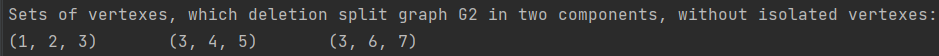
\includegraphics[width=170mm]{images/G2.png}
	
	Следующий пример --- граф, содержащий один цикл.
	
	\begin{tikzpicture}{line width=3pt}
		\def\step{1.25}
		\node[circle, draw=black] at (-2*\step, 0.5*\step) (knot1) {1};
		\node[circle, draw=black] at (-2*\step, -0.5*\step) (knot2) {2};
		\node[circle, draw=black] at (-\step, 0) (knot3) {3};
		\node[circle, draw=black] at (0 ,0) (knot4) {4};
		\node[circle, draw=black] at (\step, 0) (knot5) {5};
		
		\path[line, line width = 1.25pt] (knot1) -- (knot2);
		\path[line, line width = 1.25pt] (knot1) -- (knot3);
		\path[line, line width = 1.25pt] (knot2) -- (knot3);
		\path[line, line width = 1.25pt] (knot3) -- (knot4);
		\path[line, line width = 1.25pt] (knot4) -- (knot5);
	\end{tikzpicture}
	
	Для этого графа к нужному разделению приведет удаление только одной вершины --- точки сочленения между циклом и остальной частью графа.
	
	\begin{tabular}{|c|c|}
	\hline
	Удаленные вершины & Полученный граф \\
	\hline
	3 & \begin{tikzpicture}{line width=3pt}
		\def\step{1.25}
		\node[circle, draw=black] at (-2*\step, 0.5*\step) (knot1) {1};
		\node[circle, draw=black] at (-2*\step, -0.5*\step) (knot2) {2};
		\node[circle, draw=black] at (0 ,0) (knot4) {4};
		\node[circle, draw=black] at (\step, 0) (knot5) {5};
		
		\path[line, line width = 1.25pt] (knot1) -- (knot2);
		\path[line, line width = 1.25pt] (knot4) -- (knot5);
	\end{tikzpicture}\\
	\hline
	\end{tabular}
	
	Функция выведет тот же наборы вершин, что и в первом столбце таблицы:
	
	\lstinputlisting[linerange={17, 45-56, 84}]{graphs/tests.c} 
	
	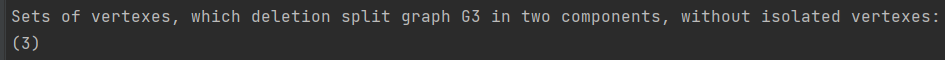
\includegraphics[width=170mm]{images/G3.png}
	
	Рассмотрим также пример графа, содержащего 2 простых цикла; точка, соединяющая их --- точка сочленения.
	
	\begin{tikzpicture}{line width=3pt}
		\def\step{1.25}
		\node[circle, draw=black] at (0, 3*\step) (knot1) {1};
		\node[circle, draw=black] at (-\step, 2*\step) (knot2) {2};
		\node[circle, draw=black] at (\step, 2*\step) (knot3) {3};
		\node[circle, draw=black] at (0, \step) (knot4) {4};
		\node[circle, draw=black] at (-\step, 0) (knot5) {5};
		\node[circle, draw=black] at (\step, 0) (knot6) {6};
		
		\path[line, line width = 1.25pt] (knot1) -- (knot2);
		\path[line, line width = 1.25pt] (knot1) -- (knot3);
		\path[line, line width = 1.25pt] (knot2) -- (knot4);
		\path[line, line width = 1.25pt] (knot3) -- (knot4);
		\path[line, line width = 1.25pt] (knot4) -- (knot5);
		\path[line, line width = 1.25pt] (knot4) -- (knot6);
		\path[line, line width = 1.25pt] (knot5) -- (knot6);
	\end{tikzpicture}
	
	Удаление точки сочленения также приводит к разделению на две простых компоненты, но так как у одной из полученных компонент больше двух вершин (и она также вырождается в линейную последовательность), можно вместе с точкой сочленения удалить и крайние вершины полученной компоненты.
	
	\begin{tabular}{|c|c|}
	\hline
	Удаленные вершины & Полученный граф \\
	\hline
	4 & \begin{tikzpicture}{line width=3pt}
		\def\step{1.25}
		\node[circle, draw=black] at (0, 3*\step) (knot1) {1};
		\node[circle, draw=black] at (-\step, 2*\step) (knot2) {2};
		\node[circle, draw=black] at (\step, 2*\step) (knot3) {3};
		\node[circle, draw=black] at (-\step, 0) (knot5) {5};
		\node[circle, draw=black] at (\step, 0) (knot6) {6};
		
		\path[line, line width = 1.25pt] (knot1) -- (knot2);
		\path[line, line width = 1.25pt] (knot1) -- (knot3);
		\path[line, line width = 1.25pt] (knot5) -- (knot6);
	\end{tikzpicture}\\
	\hline
	2, 4 & \begin{tikzpicture}{line width=3pt}
		\def\step{1.25}
		\node[circle, draw=black] at (0, 3*\step) (knot1) {1};
		\node[circle, draw=black] at (\step, 2*\step) (knot3) {3};
		\node[circle, draw=black] at (-\step, 0) (knot5) {5};
		\node[circle, draw=black] at (\step, 0) (knot6) {6};
		
		\path[line, line width = 1.25pt] (knot1) -- (knot3);
		\path[line, line width = 1.25pt] (knot5) -- (knot6);
	\end{tikzpicture}\\
	\hline
	3, 4 & \begin{tikzpicture}{line width=3pt}
		\def\step{1.25}
		\node[circle, draw=black] at (0, 3*\step) (knot1) {1};
		\node[circle, draw=black] at (-\step, 2*\step) (knot2) {2};
		\node[circle, draw=black] at (-\step, 0) (knot5) {5};
		\node[circle, draw=black] at (\step, 0) (knot6) {6};
		
		\path[line, line width = 1.25pt] (knot1) -- (knot2);
		\path[line, line width = 1.25pt] (knot5) -- (knot6);
	\end{tikzpicture}\\
	\hline
	\end{tabular}
	
	Функция выведет те же наборы вершин, что и в первом столбце таблицы:
	
	\lstinputlisting[linerange={17, 58-69, 84}]{graphs/tests.c} 
	
	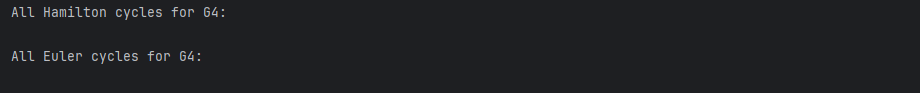
\includegraphics[width=170mm]{images/G4.png}
	
	Наконец, рассмотрим более сложный циклический граф.
	
	\begin{tikzpicture}{line width=3pt}
		\def\step{1}
		\node[circle, draw=black] at (0, 3*\step) (knot1) {1};
		\node[circle, draw=black] at (-\step, 2*\step) (knot2) {2};
		\node[circle, draw=black] at (\step, 2*\step) (knot3) {3};
		\node[circle, draw=black] at (-2*\step, \step) (knot4) {4};
		\node[circle, draw=black] at (2*\step, \step) (knot5) {5};
		\node[circle, draw=black] at (0, 0) (knot6) {6};
		
		\path[line, line width = 1.25pt] (knot1) -- (knot2);
		\path[line, line width = 1.25pt] (knot1) -- (knot3);
		\path[line, line width = 1.25pt] (knot2) -- (knot3);
		\path[line, line width = 1.25pt] (knot2) -- (knot4);
		\path[line, line width = 1.25pt] (knot3) -- (knot5);
		\path[line, line width = 1.25pt] (knot4) -- (knot5);
		\path[line, line width = 1.25pt] (knot4) -- (knot6);
		\path[line, line width = 1.25pt] (knot5) -- (knot6);
	\end{tikzpicture}
	
	В нем можно удалить только две пары вершин, чтобы полученное разделение удовлетворяло условию: 
	
	\begin{tabular}{|c|c|}
	\hline
	Удаленные вершины & Полученный граф \\
	\hline
	3, 4 & \begin{tikzpicture}{line width=3pt}
		\def\step{1}
		\node[circle, draw=black] at (0, 3*\step) (knot1) {1};
		\node[circle, draw=black] at (-\step, 2*\step) (knot2) {2};
		\node[circle, draw=black] at (2*\step, \step) (knot5) {5};
		\node[circle, draw=black] at (0, 0) (knot6) {6};
		
		\path[line, line width = 1.25pt] (knot1) -- (knot2);

		\path[line, line width = 1.25pt] (knot5) -- (knot6);
	\end{tikzpicture}\\
	\hline
	2, 5 & \begin{tikzpicture}{line width=3pt}
		\def\step{1}
		\node[circle, draw=black] at (0, 3*\step) (knot1) {1};
		\node[circle, draw=black] at (\step, 2*\step) (knot3) {3};
		\node[circle, draw=black] at (-2*\step, \step) (knot4) {4};
		\node[circle, draw=black] at (0, 0) (knot6) {6};
		
		\path[line, line width = 1.25pt] (knot1) -- (knot3);
		\path[line, line width = 1.25pt] (knot4) -- (knot6);

	\end{tikzpicture}\\
	\hline
	\end{tabular}
	
	Функция выведет те же наборы вершин, что и в первом столбце таблицы:
	
	\lstinputlisting[linerange={17, 72-84}]{graphs/tests.c} 
	
	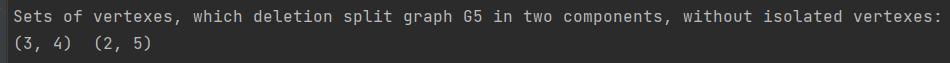
\includegraphics[width=170mm]{images/G5.png}
	
	\section{Вывод}
	\label{final}
	
	Не менее важное свойство, по которому можно классифицировать графы --- связность; оно характеризует, существует ли как минимум один путь между любой парой вершин графа. Если такой путь существует для каждой пары вершин, то граф называется связным, иначе он разделен на несколько связных компонент: их вершины связаны между собой и не связаны с другими вершинами графа. Для каждого графа можно построить бинарное отношение связности, которое отображает, существует ли путь между каждой парой вершин. Такое отношение ищется путем получения транзитивного и рефлексивного замыкания отношения, представляющего матрицу смежности исходного графа. Отношение связности обладает свойством эквивалентности и множество вершин разбито по его классам эквивалентности так же, как оно разбито на связные компоненты.
	
	Если между любой парой вершин связного графа существует только один путь (то есть в графе нет циклов), то такой граф называется деревом. Ациклический несвязный граф содержит несколько деревьев и называется лесом. Покрывающее (остовное) дерево некоторого графа --- это дерево-подграф данного графа, содержащее все его вершины. Если изначальный граф несвязный, то используется понятие покрывающего (остовного) леса --- множества покрывающих деревьев для каждой связной компоненты графа. По сути, процесс формирования такого дерева/леса сводится к удалению из исходного графа циклов (путем удаления одного из образующих цикл ребер). Для одного графа может существовать множество вариантов покрывающих деревьев/лесов, но каждое из них будет иметь одно и то же количество ребер: разность количества вершин и связных компонент исходного графа. Алгоритм Краскала описывает процесс построения одного из таких деревьев/лесов, вводя понятие <<букет>> --- множество ребер, принадлежащее одной и той же связной компоненте. 
	
	В ходе лабораторной работы реализовали на языке программирования алгоритм Краскала для построения покрывающего (остовного) леса; решили с его помощью более узкую задачу поиска всех подграфов, удовлетворяющих некоторому условию; подобрали тестовые данные для функции, решающей эту задачу, и убедились в корректности ее работы.

\end{document}